\documentclass[12pt,swedish]{article}
% För att inkludera programkoder
\usepackage[final]{pdfpages}

% Språk
\usepackage[swedish]{babel}
\usepackage[utf8]{inputenc}
\usepackage{titling}
\usepackage{listings}

% Tabell och diagram
\usepackage{booktabs}
\usepackage{float}

% Bilagor och se till att de visas på svenska
\usepackage[title,titletoc]{appendix}
\renewcommand\appendixname{Bilaga}
\renewcommand\appendixtocname{Bilagor}
\renewcommand\appendixpagename{Bilagor}

% Bilder
\usepackage{graphicx}
\graphicspath{{images/}}

% Referenser
\usepackage[style=authoryear,backend=biber,texencoding=utf8,bibencoding=utf8,natbib]{biblatex}
\usepackage{csquotes}
\addbibresource{bibliography.bib}

% Lägg till ytterligare titeldata
\postauthor{\end{tabular}\par jnikl@kth.se \par Grupp B:6\end{center}}

% Titeldata
\title{Finns det samband mellan ett programspråks ålder och dess beräkningshastighet?}
\author{Johan Niklasson}
\date{2017-11-20}


\appto\listoffigures{\addtocontents{lof}{\protect\setcounter{tocdepth}{1}}}
\appto\listoftables{\addtocontents{lot}{\protect\setcounter{tocdepth}{1}}}

% Öppna dokumentet
\begin{document}
% Så det inte blir någon sidnumrering sker på första sidan
\pagenumbering{gobble}

% Titelsida
\maketitle
\normalsize
\begin{center}

\begin{abstract}
Kan programspråk som skapades för 45 år sedan vara snabbare än programspråk som skapas idag? För att undersöka detta genomfördes ett experiment som innefattade sex olika programspråk med ett åldersspann på 37 år mellan det yngsta och det äldsta. Experimentet gick ut på att jämföra tidsåtgången i de olika språken när de löste algoritmen Collatz problem. Algoritmen kördes på en Raspberry Pi som beräknade hur lång tid respektive programspråk tog på sig att lösa problemet. Resultatet visade att programspråk har blivit snabbare med tiden, trots att vissa teorier motsätter sig detta.
\end{abstract}
\end{center}
\clearpage

% Innehållsförteckning
\tableofcontents

\listoftables
\listoffigures
\clearpage

% Börja sidnumreringen
\pagenumbering{arabic}


\section{Inledning}
Ett programspråk är en formell och strikt uppsättning av instruktioner som en dator kan läsa för att utföra uppgifter. Sedan det första programspråket utvecklades i elektroniska komponenter år 1945 \citep{bauer_wossner_1972} har det lanserats flera hundra nya programspråk. Vissa programspråk utvecklas för att lösa specifika problem - programspråket Erlang av Ericsson som exempel skapades för styrsystemen i telefonväxlar \citep{armstrong_1997}. Andra språk, såsom Scratch, har tagits fram i undervisningssyfte för barn \citep{maloney_resnick_rusk_silverman_eastmond_2010}.

Men även då vissa programspråk har haft vissa typer av uppgifter i hänsyn vid sin framtagning, har dessa då samtidigt lyckats bli snabbare? Moores Lag som beskriver att antalet transistorer på chip växer potentiellt, resulterar i datorer och processorer blir snabbare varje år \citep{schaller_1997}. Kan det därför finnas ett mindre behov av att nyare programspråk inte behöver vara lika snabba utan kanske istället till exempel mer lättlästa för människor?

\subsection{Syfte}
Syftet med studien är att ta fram ett underlag om varför nya programspråk skapas. Då det kan vara flera egenskaper som påverkar framtagningen och användningen av programspråk har ett fokus koncentrerats på en av dessa - beräkningshastigheten hos ett programspråk.

\subsection{Frågeställning}
Frågeställningen för studien är: “Finns det någon korrelation i beräkningshastighet och utgivningsår för mellannivåspråk?”

\subsection{Avgränsning}
I studien är det enbart intressant att jämföra språk med liknande egenskaper. Därför kommer kompilerbara mellannivåspråk att testas som går att exekveras (köras) och kompileras på en Raspberry Pi (en liten dator i storlek av ett kreditkort).


\section{Begrepp}
I studien används ett antal termer som är relevanta för experimentet. I detta avsnitt kommer de förklaras på ett förenklat sätt som är relevant för studien.

\subsection{Programkod}
En programkod är en uppsättning instruktioner som utförs av en dators processor. Instruktionerna består av jämförelser eller matematiska operationer av två värden som sedan utför efterföljande instruktioner beroende på resultatet.

\subsection{Processor}
Processorn brukar hänvisas som “hjärnan” i en dator som utför de flesta av instruktionerna från programkod \citep{charuba_1996}. Den här studien kommer enbart fokusera på tiden för de beräkningar som processorn utför.

\subsection{Kompilering}
Att kompilera en programkod innebär att programkoden skrivs om från beskrivande syntaxer till maskinkod som processorn kan läsa. I programmeringsspråk brukar en så kallad IF-sats, som kontrollerar villkor, skrivas som följande:
\begin{lstlisting}
IF condition THEN
    sequence 1
ELSE
    sequence 2
ENDIF
\end{lstlisting}
Detta är inte programkod som processorn kan tolka utan måste först skrivas om till instruktioner den kan förstå. Denna omskrivning kallas för kompilering. Ett program som kallas för kompilator gör just detta och skriver om den programkoden till det förväntade formatet, så kallad maskinkod \citep{srikant_shankar_2008}.

\subsection{Nivåer på programspråk}
Inom programmering är det skillnad på hur programspråk fungerar när de exekveras. I studien kommer enbart mellannivåspråk att användas.
\begin{description}
    \item [Mellannivåspråk:] I ett mellannivåspråk kompileras programkoden innan den exekveras. Det kan liknas med att samtliga instruktioner läses en enda gång och utförs sedan direkt efter varandra.
    \item [Högnivåspråk:] Ett högnivåspråk kompilerar programkoden samtidigt som instruktionerna utförs. Det innebär att varje instruktion läses precis innan den utförs och resulterar därför i att programkoden exekveras långsammare än i ett mellannivåspråk \citep{maclachlan_1992}.
\end{description}

\subsection{Collatz problem}
Collatz problem är ett olöst matematiskt problem inom talteorin. Problemet beskriver ett sätt utföra ett antal matematiska steg i följd för att till slut nå talet ett. Stegen är följande:
\begin{enumerate}
    \item [1.] Välj ett positivt heltal \( n \) som är större än ett.
    \item [2.] Om \( n \) är jämnt, dividera det med två. Om \( n \) är udda, multiplicera det med tre och addera ett.
    \item [3.] Repetera steg två tills \( n \) når ett.
\end{enumerate}
I studien kommer detta problem skrivas om till en algoritm som utför stegen ovan för enskilda tal. Algoritmen används sedan för att utföra instruktioner som går att mäta i tid mellan olika programspråk. Algoritmen använder enbart addition, multiplikation, division som matematiska operationer.

Algoritmen är oförutsägbar för olika tal då det inte finns något mönster för hur många iterationer som krävs innan talet når ett. Detta har dock ingen inverkan i jämförelser mellan olika programspråk så länge samma tal jämförs, eftersom samma tal alltid genererar samma antal steg.

\subsection{Raspberry Pi}
Raspberry Pi är en liten dator i storlek av ett kreditkort och använder operativsystemet Linux som är brett använt inom programmering. Datorn är lämplig för tester då den har få processer och program som påverkar tidsmätningar, jämfört med till exempel en PC  \citep{andrews_2013}.


\newpage
\section{Metod}
Ett initialt urval på programspråk gjordes från \citetitle{tiobe} (\citeyear{tiobe}) som listar de 25 mest populära programspråken, vilka går att finna i bilaga \ref{appendix:languages}. Urvalet gjordes för att få ett uppsättning språk som faktiskt används av företag och utvecklare. Av dessa 25 språk var det cirka hälften som var mellannivåspråk och ytterligare en halvering skedde efter att ha filtrerat bort de språk som inte var kompatibla med en Raspberry Pi. Språken med sina respektive utgivningsår som återstod blev då följande:

\begin{itemize}
    \item C (1972)
    \item Ada (1980)
    \item C++ (1983)
    \item Java (1995)
    \item D (2001)
    \item Go (2009)
\end{itemize}
För att jämföra olika språk med varandra behövdes en typ av problem lösas. Problemet som användes i studien var Collatz problem som utförde olika matematiska operationer sekventiellt. Totalt användes sex språk, kategoriserade utifrån sitt utgivningsår.

Problemet programmerades som en algoritm i de olika språken (se bilaga \ref{appendix:programcodes}), kompilerades och exekverades därefter under tidsmätning. Algoritmen körde alla tal mellan 2 till 100 000, och gjorde detta 100 gånger om, då ju längre tid algoritmen tog på sig, desto noggrannare blev jämförelsen mellan språken. För att få fram ett mätvärde i tid användes en inbyggd timer i en Raspberry Pi som angav tiden i millisekunder.


\newpage
\section{Resultat}
Nedan presenteras de resultat som experimentet genererade. Alla tidsmätningar som presenteras anges i sekunder med tre decimaler.

% Tabell med rådata
\begin{table}[H]
Tabell \ref{table:result} presenterar de värden som uppmättes i de olika körningarna i experimentet. Populariteten är hämtad från \citetitle{tiobe} (\citeyear{tiobe}), samma källa som för urvalet av programspråken. Den procentuella populariteten mäts i antal sökträffar språket genererar i sökmotorer delat på totala antalet träffar för alla språk tillsammans.

Från datan i tabell \ref{table:result} kan det utläsas att det äldsta språket C i studien var långsammast medan det nyaste språket Go var snabbast. Ändå är C det näst mest populära språket på cirka 7.7\% medan Go har en popularitet på ungefär 2\%.
\begin{center}
\caption{Mätvärden och popularitet}
\label{table:result}
\begin{tabular}{@{}llll@{}}
\toprule
Utgivningsår & Programspråk & Exekveringstid & Popularitet \\ \midrule
1972         & C            & 5.000 s        & 7.74\%      \\
1980         & Ada          & 4.452 s        & 0.78\%      \\
1983         & C++          & 4.744 s        & 5.18\%      \\
1995         & Java         & 3.312 s        & 16.38\%     \\
2001         & D            & 4.440 s        & 1.23\%      \\
2009         & Go           & 2.980 s        & 1.98\%      \\ \bottomrule
\end{tabular}
\end{center}
\end{table}

% Diagram med beräkningshastighet
\begin{figure}[H]
\begin{center}
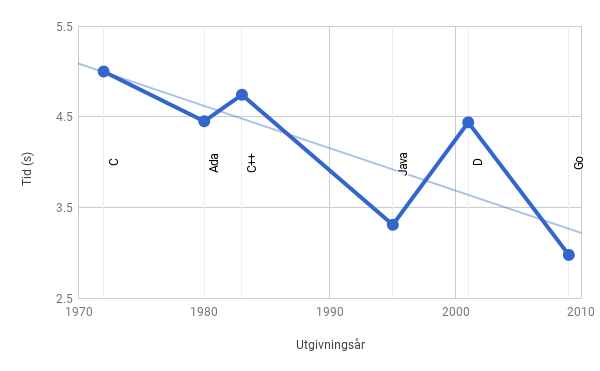
\includegraphics[width=1\textwidth,natwidth=600,natheight=371]{performance.png}
\caption{Exekveringstid över utgivningsår}
\label{figure:performance}
\end{center}
Figur \ref{figure:performance} visar ett diagram med exekveringstiden för de olika programspråken över sitt utgivningsår. Figuren visar även en trendlinje som anger riktning på exekveringstidernas utveckling över utgivningsåren. Ju lägre punkt och siffra desto snabbare är språket.
\end{figure}

% Diagram med popularitet
\begin{figure}[H]
\begin{center}
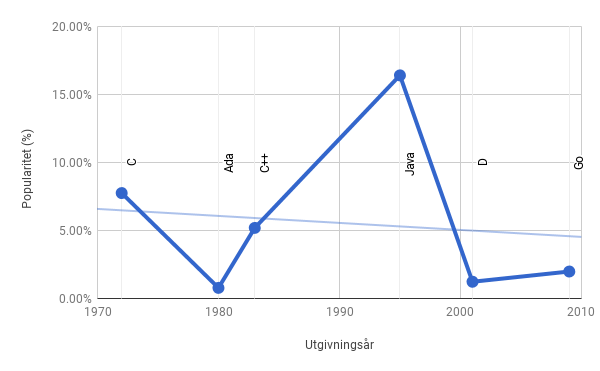
\includegraphics[width=1\textwidth,natwidth=600,natheight=371]{popularity.png}
\caption{Popularitet över utgivningsår}
\label{figure:popularity}
\end{center}
Figur \ref{figure:popularity} presenterar i tidsordning populariteten för de olika programspråken över sitt utgivningsår, i samma horisontella skala som i figur \ref{figure:performance}. Java är mest populär med strax över 16\% och utgivningsår 1995, 14 år äldre och 8 gånger mer populärt än språket Go. Det äldsta språket C hade en popularitet på cirka 7.7\% och därmed det näst mest populära språket i studien. Ett högt värde i grafen innebär ett mer populärt språk.
\end{figure}


\section{Diskussion}
Om enbart trendlinjen i figur \ref{figure:performance} beaktas kan en logisk följd dras att det är en fallande trend, det vill säga att exekveringstiden i programspråk blir snabbare med tiden. Ändå är det långsammaste språket C det näst mest populära språket på cirka 7.7\%, jämfört med Go som var snabbast men endast hade en popularitet på ungefär 2\%. Detta kan naturligtvis bero på att C har funnits i 37 år längre än Go och därför hunnit användas till fler applikationer.

I figur \ref{figure:popularity}, där programspråkens popularitet visas, blir sambanden inte lika tydliga. Att Ada och D är såpass långt ner i grafen skulle kunna resoneras från deras långsamma beräkningshastighet, vilket dock motsätts med C++ som är långsammare men över dubbelt så populärt som både D och Ada tillsammans. Det populäraste programspråket är Java med strax över 16\%, 23 år yngre och mer än två gånger populärare än C som är näst mest populärt. En bidragande faktor till Javas popularitet kan troligtvis härledas till att operativsystemet Android och dessa appar bygger på samma språk \citep{gruman_2017}.

När nyare programspråk lanseras har de en högre förväntan på sig att kunna utföra fler avancerade operationer utan att utvecklaren själv behöver skriva koden \citep{stroustrup_1997}. Detta gör att kodbasen (programspråkets byggstenar) för språken måste innehålla fler funktioner och operationer som tynger ner programmet, men lyckas ändå bli snabbare med tiden - ett resultat som  \citeauthor{luong_2017} (\citeyear{luong_2017}) motsätter sig där han diskuterar varför vissa språk är snabbare än andra. \citeauthor{luong_2017} påstår att äldre språk, såsom C och C++, är snabbare av just den anledningen - att de är nedskalade och utför endast det de programmeras till.

Studien hade kunnat visat ett annat resultat om ett större urval av mellannivåspråk använts. Om dessutom separata tester på högnivåspråk hade inkluderats skulle dessa kunnat stärka eller motbevisa resultatet. Kompilatorn för programspråk har även en viss inverkan i hur snabbt det kompilerade programmet blir \citep{srikant_shankar_2008}, något som inte tagits hänsyn till i den här studien. Även fler typer av algoritmer skulle kunna testats för att bekräfta respektive programspråks beräkningshastighet.


\section{Slutsats}
Syftet med studien har varit att testa om beräkningshastigheten i programspråk har ett samband med hur gamla de är med hjälp av olika experiment. Trenden som visar att programspråken blir snabbare i sin beräkningshastighet med tiden skulle kunna ses som självklar då det finns mer vetskap för att utveckla programspråk idag än för 45 år sedan då C först kom. Ett exempel på samma utveckling är att bilar blivit snabbare under samma tidsperiod. Programspråken har växt med fler operationer och funktioner, trots det har de inte blivit långsammare; utan tvärtom, blivit snabbare, vilket studien redovisat för.

Frågeställningen har besvarats, även om det finns fler aspekter att tillämpa för att få ett bredare resultat och ett starkare bevis på att trenden stämmer.

% Skriv ut referenser i innehållsförteckningen
\addcontentsline{toc}{section}{Referenser}
\printbibliography

% Rensa sidan, och ta bort sudnumreringen efter bilagor börjar
\clearpage
\begin{appendices}
\pagenumbering{gobble}

% Göm subsections, det blir bara plottrigt här
\addtocontents{toc}{\protect\setcounter{tocdepth}{1}}

% Bilaga med programspråk
\section{Urval av programspråk}\label{appendix:languages}
\begin{table}[H]
\centering
\label{appendix:table:languages}
\begin{tabular}{lll}
\toprule
Placering & Programspråk         & Popularitet \\ \midrule
1         & Java                 & 16.38\%     \\
2         & C                    & 7.74\%      \\
3         & C++                  & 5.18\%      \\
4         & C\#                  & 4.41\%      \\
5         & Python               & 3.92\%      \\
6         & Visual Basic .NET    & 3.17\%      \\
7         & PHP                  & 3.01\%      \\
8         & JavaScript           & 2.67\%      \\
9         & Delphi/Object Pascal & 2.54\%      \\
10        & Swift                & 2.27\%      \\
11        & Perl                 & 2.26\%      \\
12        & Ruby                 & 2.25\%      \\
13        & Assembly language    & 2.23\%      \\
14        & R                    & 2.02\%      \\
15        & Visual Basic         & 2.01\%      \\
16        & Objective-C          & 2.00\%      \\
17        & Go                   & 1.98\%      \\
18        & MATLAB               & 1.85\%      \\
19        & PL/SQL               & 1.67\%      \\
20        & Scratch              & 1.47\%      \\
21        & SAS                  & 1.29\%      \\
22        & D                    & 1.23\%      \\
23        & Dart                 & 1.20\%      \\
24        & ABAP                 & 1.15\%      \\
25        & Ada                  & 0.78\%      \\ \bottomrule
\end{tabular}
\end{table}

\clearpage

\section{Programkoder}\label{appendix:programcodes}

\lstset{basicstyle=\ttfamily\scriptsize,
        keywordstyle=\color{blue}\ttfamily,
        stringstyle=\color{red}\ttfamily,
        commentstyle=\color{green}\ttfamily,
        breaklines=true
}

\subsection{Ada}
\begin{lstlisting}[language=ada]
with Gnat.Io; use Gnat.Io;
procedure col is
    function collatz(n1: Integer) return Integer is
        c: Integer;
        n: Integer;
    begin
        n := n1;
        c := 0;

        while n /= 1 loop
            if n mod 2 = 0 then
                n := n / 2;
            else
                n := n * 3 + 1;
            end if;
            c := c + 1;
        end loop;

        return c;
    end;

   f: Integer;
begin
    f := 0;

    for j in Integer range 1 .. 100 loop
        for i in Integer range 1 .. 100000 loop
            f := f + collatz(i);
        end loop;
    end loop;

    Put(f);
    New_Line;
end col;
\end{lstlisting}


\newpage
\subsection{C}
\begin{lstlisting}[language=c]
#include <stdio.h>


int collatz(int);

int main()
{
    int f = 0;
    int i;
    int j;

    for (j = 0; j < 100; j++)
    {
        for (i = 1; i <= 100000; i++)
        {
            f = f + collatz(i);
        }
    }

    printf("%d\n", f);

    return 0;
}

int collatz(int n)
{
    int c = 0;

    while (n != 1)
    {
        if (n % 2 == 0)
        {
            n = n / 2;
        }
        else
        {
            n = n * 3 + 1;
        }
        c = c + 1;
    }

    return c;
}
\end{lstlisting}


\newpage
\subsection{C++}
\begin{lstlisting}[language=c++]
#include <iostream>
using namespace std;

int collatz(int);

int main()
{
    int f = 0;
    int i;
    int j;

    for (j = 0; j < 100; j++)
    {
        for (i = 1; i <= 100000; i++)
        {
            f = f + collatz(i);
        }
    }

    cout << f << endl;

    return 0;
}

int collatz(int n)
{
    int c = 0;

    while (n != 1)
    {
        if (n % 2 == 0)
        {
            n = n / 2;
        }
        else
        {
            n = n * 3 + 1;
        }
        c = c + 1;
    }

    return c;
}
\end{lstlisting}


\newpage
\subsection{D}
\begin{lstlisting}[language=C]
import std.stdio;

int main()
{
    int f = 0;
    int i;
    int j;

    for (j = 0; j < 100; j++)
    {
        for (i = 1; i <= 100000; i++)
        {
            f = f + collatz(i);
        }
    }

    writeln(f);

    return 0;
}

int collatz(int n)
{
    int c = 0;

    while (n != 1)
    {
        if (n % 2 == 0)
        {
            n = n / 2;
        }
        else
        {
            n = n * 3 + 1;
        }
        c = c + 1;
    }

    return c;
}
\end{lstlisting}

\newpage
\subsection{Go}
\begin{lstlisting}[language=Python]
package main

import (
    "fmt"
)

func main() {
    f := 0

    for j := 0; j < 100; j++ {
        for i := 1; i <= 100000; i++ {
            f = f + collatz(i)
        }
    }

    fmt.Println(f)
}

func collatz(n int) int {
    c := 0

    for n > 1 {
        if n % 2 == 0 {
            n = n / 2
        } else {
            n = 3 * n + 1
        }
        c = c + 1
    }

    return c
}
\end{lstlisting}


\newpage
\subsection{Java}
\begin{lstlisting}[language=java]
public class col
{
    public static void main(String[] args)
    {
        int f = 0;
        int i;
        int j;

        for (j = 0; j < 100; j++)
        {
            for (i = 1; i <= 100000; i++)
            {
                f = f + collatz(i);
            }
        }

        System.out.println(f);
    }

    public static int collatz(int n)
    {
        int c = 0;

        while (n != 1)
        {
            if (n % 2 == 0)
            {
                n = n / 2;
            }
            else
            {
                n = n * 3 + 1;
            }
            c = c + 1;
        }

        return c;
    }
}
\end{lstlisting}

\end{appendices}

% Stäng dokumentet
\end{document}
